% PREAMBLE ====
\documentclass[preprint,3p,twocolumn]{elsarticle} % TODO: What model?

% Use times font
\usepackage{pslatex}

% Math
\usepackage{amsmath}

% Tables, Figures
\usepackage{booktabs}
\usepackage{threeparttable}
\usepackage{float}
\usepackage{caption}
\setlength{\tabcolsep}{10pt}

% Graphics
\usepackage{graphicx}
\DeclareGraphicsExtensions{.pdf,.png}
\graphicspath{{../../figures/}}

% References
\usepackage{numcompress}
\biboptions{super}
\bibliographystyle{model3-num-names}

% DOCUMENT ====
\begin{document}
% FRONTMATTER ====
\begin{frontmatter}
\title{Parkinson's disease cluster analysis}
\author[c3]{Pablo Martinez-Martin}
\ead{pmartinez@isciii.es}
\author[bc]{Jesse Mu}
\ead{muj@bc.edu}
\author[cig]{Concha Bielza}
\ead{mcbielza@fi.upm.es}
\author[cig]{Pedro Larra\~naga}
\ead{plarranaga@fi.upm.es}
\address[c3]{Area of Applied Epidemiology, National Centre of Epidemiology and CIBERNED, Carlos III Institute of Health, Madrid, Spain}
\address[bc]{Department of Computer Science, Boston College, Chestnut Hill, Massachusetts, USA}
\address[cig]{Computational Intelligence Group, Polytechnic University of Madrid, Madrid, Spain}

\begin{abstract}
\emph{Background} \quad This is the background. \\
\emph{Methods} \quad  These are methods. \\
\emph{Findings} \quad These are findings. \\
\emph{Interpretation} \quad This is interpretation. \\
\emph{Funding} \quad This is funding.
\end{abstract}
\journal{The Lancet Neurology}
\end{frontmatter}

% BODY ====

\section{Introduction}

\section{Methods}

\subsection{Statistical analysis}

Out of the 951 patients in the study, we used listwise deletion to exclude 50 patients due to
missing measurements in the variables of interest, resulting in 901 remaining patients. All
symptoms were scaled to $z$-scores ($\mu = 0$, $\sigma = 1$) before clustering, and unscaled
afterwards. Analysis was conducted in R 3.2.4 (www.r-project.org).

\subsubsection{Cluster analysis}

$k$-means was used for cluster analysis. We performed two analyses on the
patients in the dataset: the first on the nine aggregate nonmotor symptom
domains and the four motor symptoms, and the second on the 30 individual
nonmotor symptoms collected with the four motor symptoms. Complete-linkage
hierarchical clustering on the 30 nonmotor symptoms was also performed to observe the
categorization of symptoms.

\subsubsection{Determining $k$}

Various formal measures were used to determine the optimal number of
clusters for the dataset. First, the optimal $k$ according to the Gap Statistic and the
1-standard-error method\cite{tibshirani01gap} was $k = 4$ (Figure~\ref{fig:gap}). Second, although
the globally-optimal clusters reported from stability measures of the clValid R package
\cite{brock11clvalid} stability are 2, 6, and 8 (Figure~\ref{fig:stability}), there appeared to be
consensus that $k = 4$ is a locally-optimal number of clusters which supported the gap statistic
result.

Other cluster validation methods (SSE scree plot, minimum average silhouette width) generally
suggested 2 clusters. As a consequence, $k = 2, 3, 4$ was tried, where $k = 2, 3$ simply divided
the data uninformatively into groups with varying levels of overall PD severity. Thus $k = 4$ was
selected to offer a good blend of model fit, informativeness, and parsimony.

\begin{figure}[h]
  \centering
  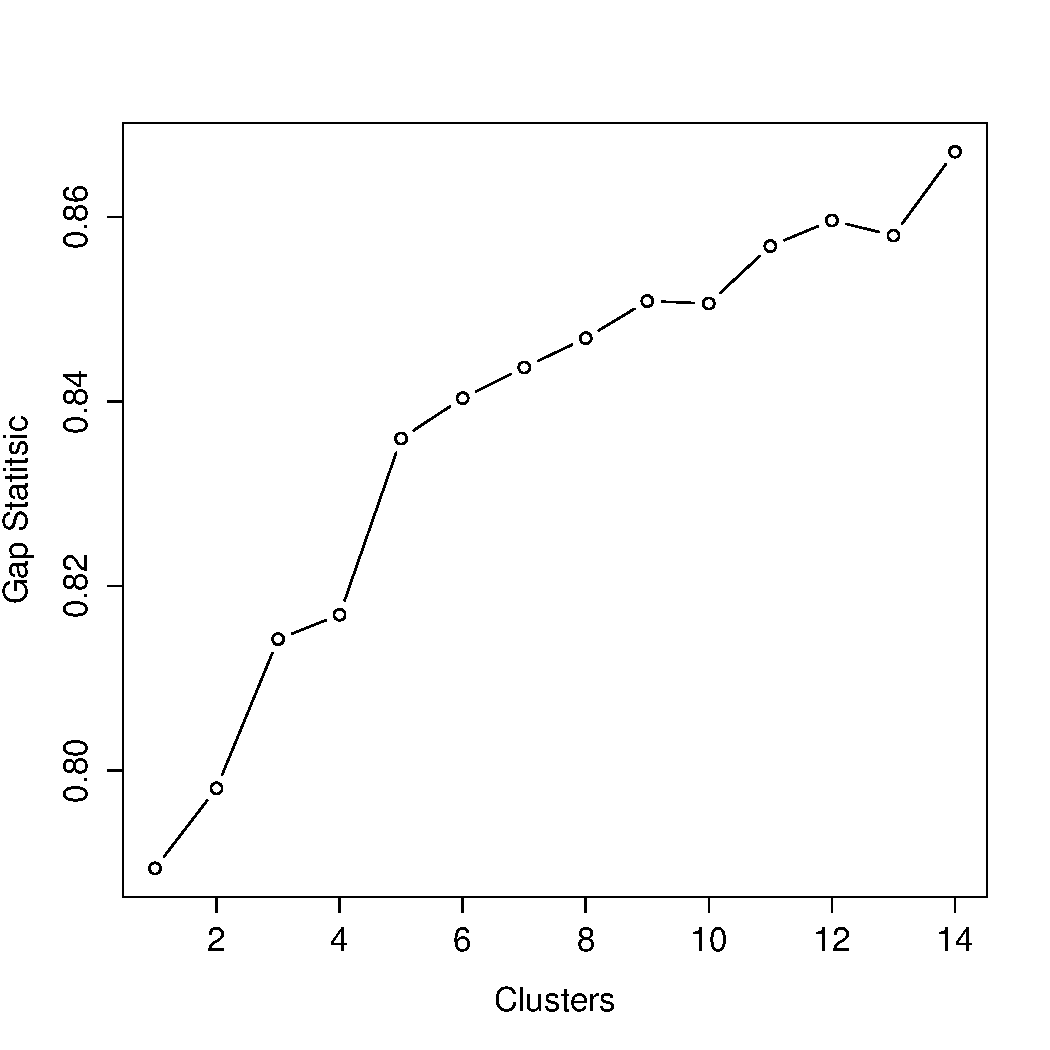
\includegraphics[width=\linewidth]{gap-statistic.pdf}
  \caption{Plot of gap statistic versus number of clusters with $k$-means on 100 bootstrapped
    samples. Error bars are standard error. Per the method described in\cite{tibshirani01gap}, 4 is the smallest $k$ such
    that $\text{Gap}(k) \geq \text{Gap}(k + 1) - \text{se}_{k + 1}$.}
  \label{fig:gap}
\end{figure}

\begin{figure}[h]
  \centering
  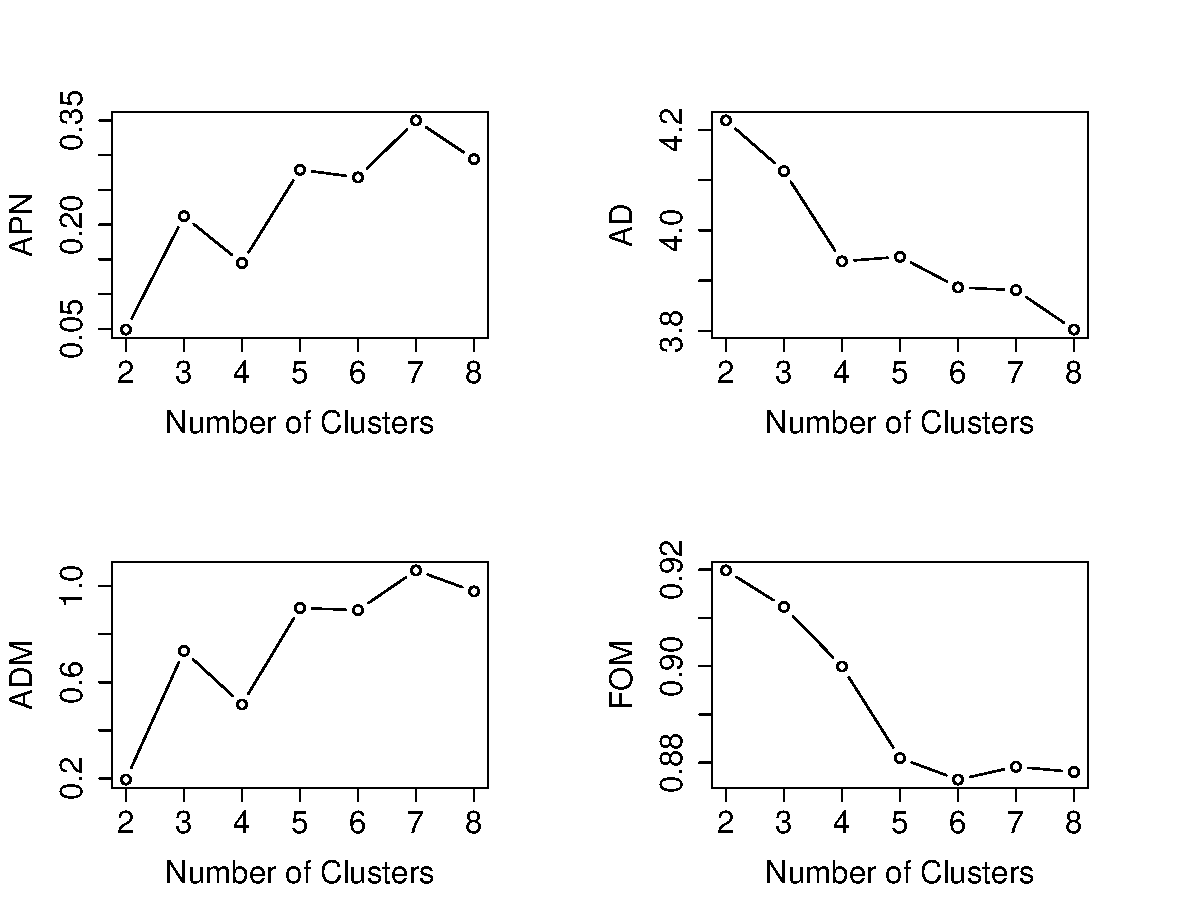
\includegraphics[width=\linewidth]{stability-measures.pdf}
  \caption{Average proportion of non-overlap (APN), average distance (AD), average distance
    between means (ADM), and figure of merit (FOM) stability measures\cite{datta2006methods,
    yeung2001validating}. Statistics should be minimized; notice the local optima at $k = 4$ for
  APN, AD, and ADM.}
  \label{fig:stability}
\end{figure}

\subsubsection{Interpretation}

For the clustering on nonmotor domains, we displayed the distribution of each symptom for the four
clusters using boxplots, which allowed us to visualize the center and spread of each cluster. Since
the number of variables was larger for the clustering on the individual symptoms, we visualized
results for the second analysis with a heatmap. Finally, for the hierarchical clustering on the
symptoms themselves, we displayed results in a dendrogram and clustered the symptoms into four
interpretable clusters.

For each symptom in both clusterings, we used one-way ANOVA to test the equality of symptom means
across the clusters found, using Bonferroni correction for multiple testing with corrected $p <
0.05$ considered significant. Differences among pairwise clusters were tested post-hoc using
Tukey's range test.

\section{Results}

\subsection{Clustering with nonmotor domains}

$k$-means clustering on the nine nonmotor domains and the four motor symptoms found four clusters,
available in Table~\ref{tab:nmd} with boxplots in Figure~\ref{fig:box}. Cluster means for all
symptoms were found to be statistically different, with specific pairwise differences noted in the table.

Cluster 1 ($n = 406$) patients were mildly affected in all domains.

Cluster 2 ($n = 189$) patients were severely
affected in nonmotor domains but mildly affected in motor domains (Nonmotor-Dom), cluster 3 ($n =
221$) patients were severely affected in motor domains but mildly affected in nonmotor domains
(Motor-Dom), and cluster 4 ($n = 88$) patients were severely affected in all domains. Statistics
for variables not used in the clustering were explored in Table~\ref{tab:nmd_extra}.

\begin{table*}[t]
  \centering
  \caption{Summaries of clustering on nonmotor domains. Bold indicates the highest score for that
  symptom out of the four clusters.}
  \label{tab:nmd}
  \begin{threeparttable}
  \begin{tabular}{l r r r r}
    \toprule
    Cluster & 1 & 2 & 3 & 4 \\
    $n$ & 406 (44.9\%) & 189 (20.9\%) & 221 (24.4\%) & 88 (9.7\%) \\
    \midrule
    \textbf{Nonmotor} (Domains) & & & & \\
    Cardiovascular (0--24) & 0.7 (1.6)\tnote{24} & 2.3 (2.9)\tnote{134} & 1.1 (2.0)\tnote{24} &
    \textbf{7.0} (6.0)\tnote{234} \\
    Sleep/fatigue (0--48) & 4.3 (4.8)\tnote{234} & 14.9 (8.2)\tnote{134} & 6.9 (6.3)\tnote{124}
    & \textbf{21.0} (10.0)\tnote{123} \\
    Mood/cognition (0--60) & 3.1 (4.5)\tnote{234} & 16.1 (14.0)\tnote{134} & 6.6
    (8.1)\tnote{124} & \textbf{23.4} (14.3)\tnote{123} \\
    Perception/hallucination (0--36) & 0.5 (1.7)\tnote{24} & 1.9 (3.5)\tnote{134} & 0.8
    (2.0)\tnote{24} & \textbf{8.6} (6.9)\tnote{123} \\
    Attention/memory (0--36) & 2.8 (4.2)\tnote{24} & 8.9 (8.1)\tnote{134} & 3.2 (4.4)\tnote{24} &
    \textbf{15.6} (11.1)\tnote{123} \\
    Gastrointestinal (0--36) & 2.8 (3.9)\tnote{234} & 8.8 (7.1)\tnote{134} & 4.1
    (4.7)\tnote{124} & \textbf{14.6} (9.6)\tnote{123} \\
    Urinary (0--36) & 4.5 (5.9)\tnote{234} & 12.4 (9.7)\tnote{134} & 6.1 (6.4)\tnote{124} &
    \textbf{20.3} (9.9)\tnote{123} \\
    Sexual function (0--24) & 1.5 (3.1)\tnote{24} & 6.4 (7.4)\tnote{134} & 2.5 (4.1)\tnote{24} &
    \textbf{9.0} (9.7)\tnote{123} \\
    Miscellaneous (0--48) & 3.9 (4.7)\tnote{24} & 13.2 (8.6)\tnote{13} & 5.2 (5.8)\tnote{24} &
    \textbf{14.0} (9.5)\tnote{13} \\
    \midrule
    \textbf{Motor} & & & & \\
    Tremor & 1.9 (1.8)\tnote{34} & 1.6 (1.9)\tnote{34} & \textbf{4.3} (2.8)\tnote{124} & 3.5
    (3.8)\tnote{123} \\
    Bradykinesia & 1.5 (0.9)\tnote{234} & 2.1 (1.1)\tnote{134} & 3.6 (0.9)\tnote{124} &
    \textbf{4.0} (1.5)\tnote{123} \\
    Rigidity & 1.5 (0.9)\tnote{234} & 1.8 (1.1)\tnote{134} & 3.3 (0.9)\tnote{124} &
    \textbf{3.8} (1.4)\tnote{123} \\
    Axial & 1.8 (1.6)\tnote{234} & 3.3 (2.1)\tnote{134} & 4.3 (2.4)\tnote{124} &
    \textbf{7.4} (2.9)\tnote{123} \\
    \bottomrule
  \end{tabular}
  \begin{tablenotes}
    \small
    \item[1] Significant difference with cluster 1 ($p < 0.05$)
    \item[2] Significant difference with cluster 2 ($p < 0.05$)
    \item[3] Significant difference with cluster 3 ($p < 0.05$)
    \item[4] Significant difference with cluster 4 ($p < 0.05$)
    \item[\textdagger] Another footnote.
  \end{tablenotes}
  \end{threeparttable}
\end{table*}

\begin{figure*}[b]
  \centering
  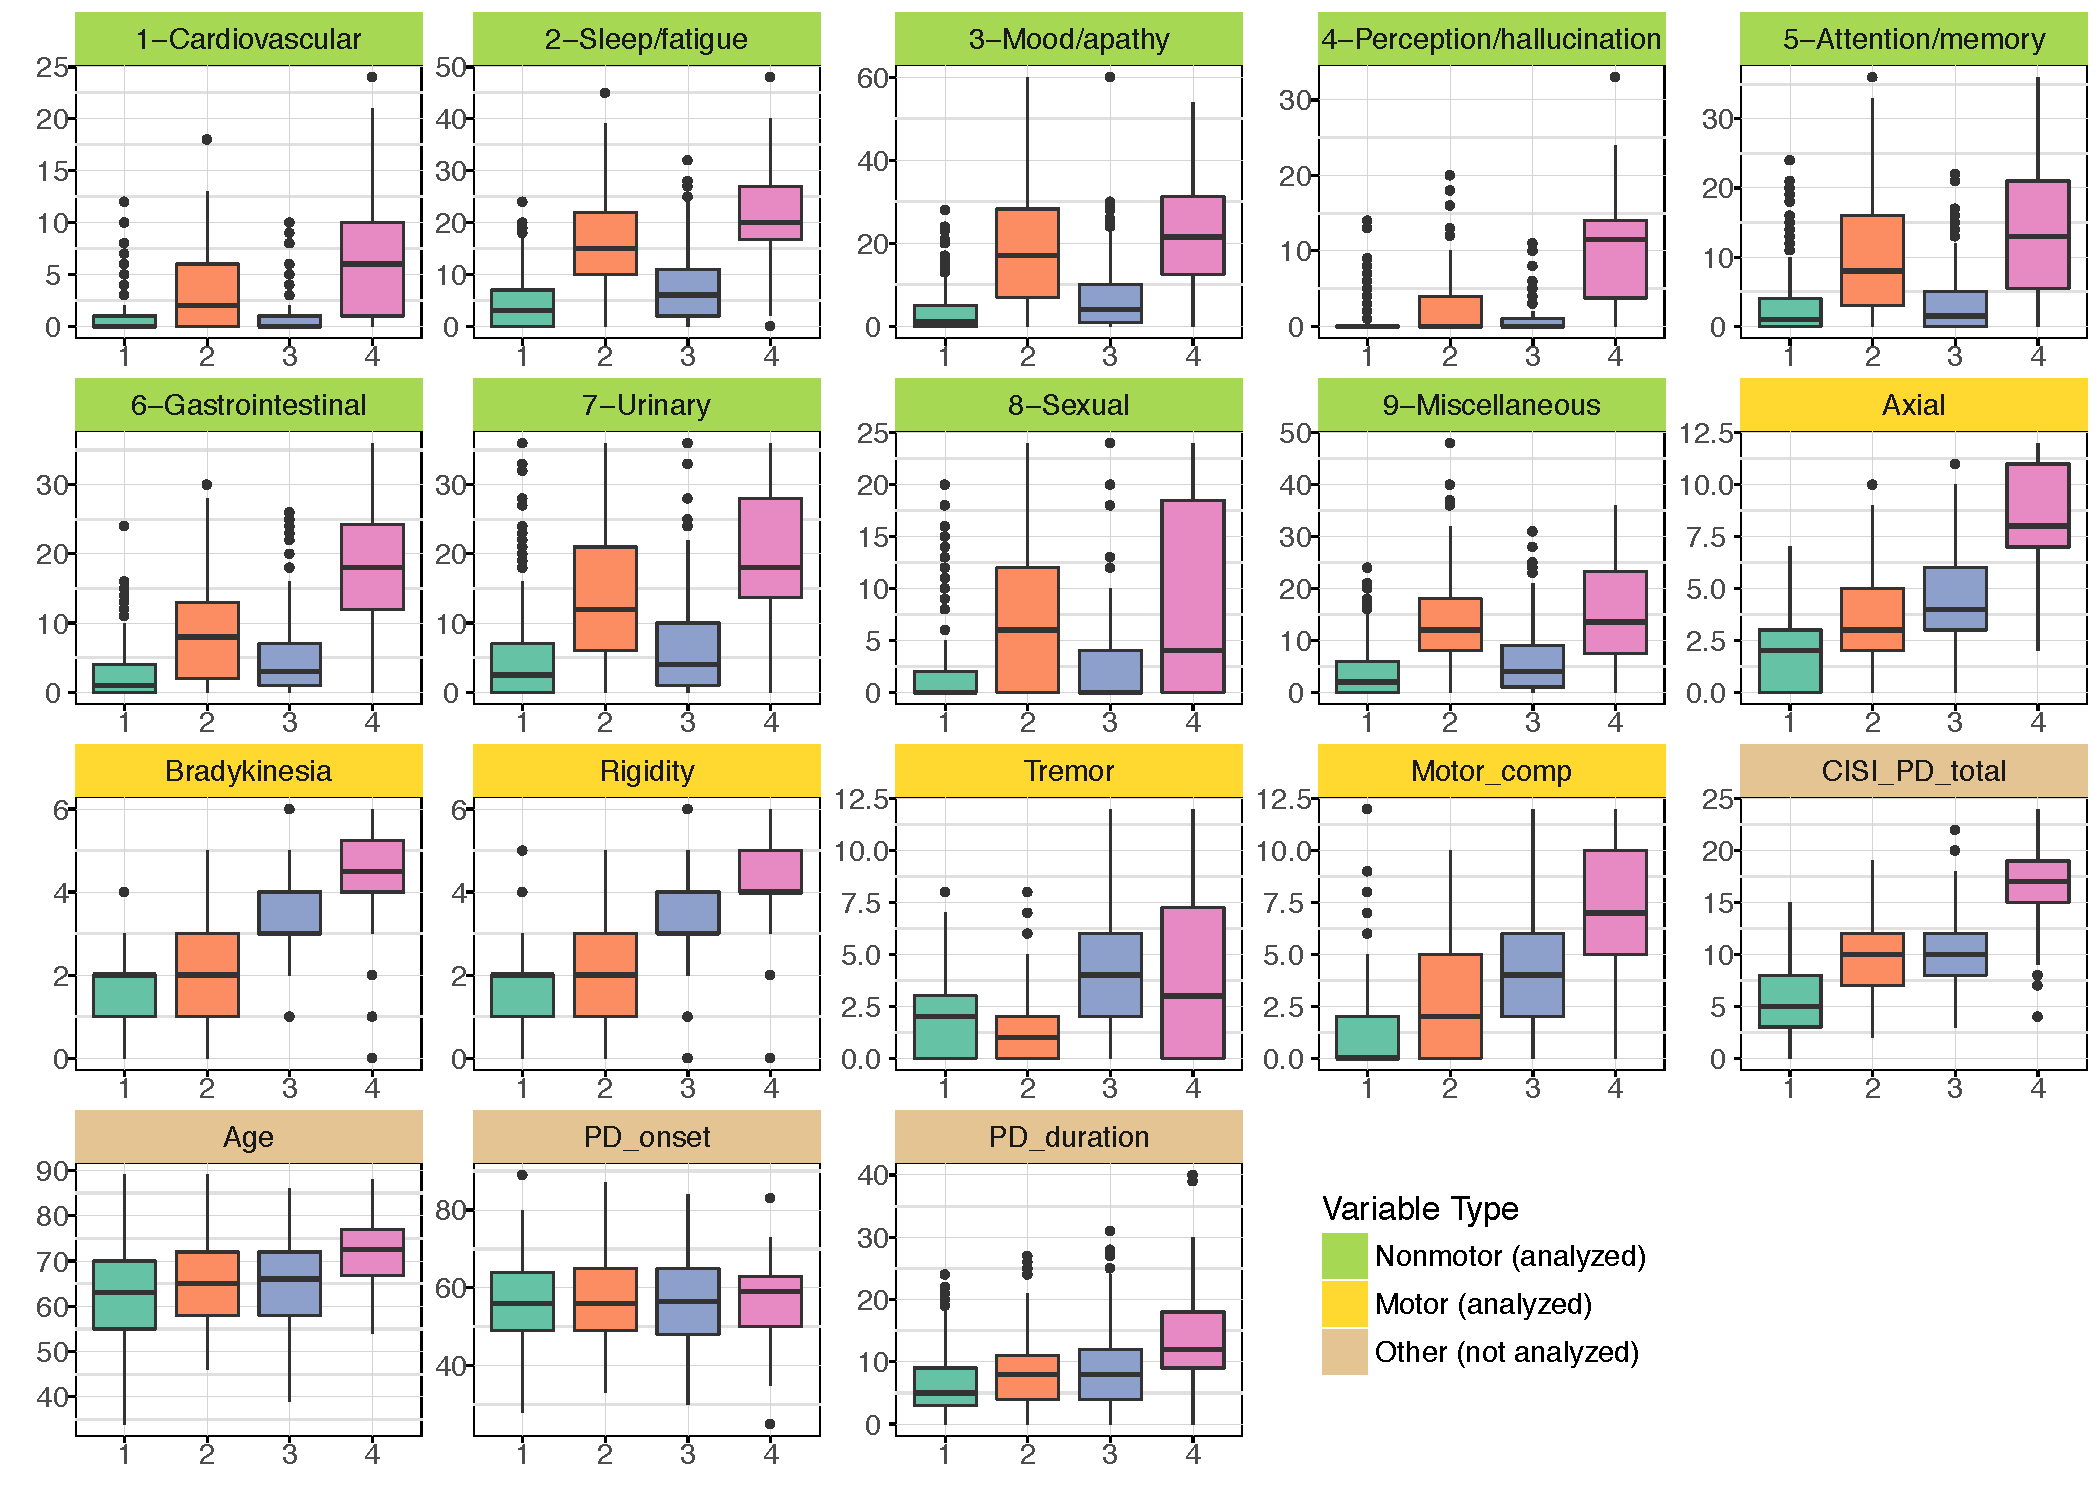
\includegraphics[width=\linewidth]{kmeans-summaries-4-pub.pdf}
  \vspace{-7.5em}
  \captionsetup{justification=raggedleft,
    singlelinecheck=false
  }
  \caption{Boxplot summaries for clusters found \\ when clustering with nonmotor domains.}
  \label{fig:box}
\end{figure*}

\begin{table*}[t]
  \centering
  \caption{Cluster statistics for variables not used in the analysis}
  \label{tab:nmd_extra}
  \begin{threeparttable}
  \begin{tabular}{l r r r r}
    \toprule
    & 1 & 2 & 3 & 4 \\
    \midrule
      Age & 62.7 (9.7) & 64 (9) & 65 (10.2) & 70.5 (8.9) \\
      Sex & 0.4 (0.5) & 0.5 (0.5) & 0.3 (0.5) & 0.4 (0.5) \\
      PD\_Onset & 56 (10.6) & 55.2 (10.1) & 56.9 (11.1) & 58.2 (11.4) \\
      PD\_Duration & 6.7 (4.8) & 8.7 (5.7) & 8 (5.5) & 12.3 (8.1) \\
      CISI\_Total & 5.7 (3.2) & 9.2 (3.9) & 9.7 (3.5) & 14.8 (5.1) \\
      Surgery & 0 (0.2) & 0.1 (0.2) & 0 (0.2) & 0 (0.1) \\
    \bottomrule
  \end{tabular}
  \begin{tablenotes}
    \small
    \item[1] Significant difference with cluster 1 ($p < 0.05$)
    \item[2] Significant difference with cluster 2 ($p < 0.05$)
    \item[3] Significant difference with cluster 3 ($p < 0.05$)
    \item[4] Significant difference with cluster 4 ($p < 0.05$)
    \item[\textdagger] Another footnote.
  \end{tablenotes}
  \end{threeparttable}
\end{table*}
\subsection{Clustering with nonmotor symptoms}

\subsection{Hierarchical clustering on symptoms}

Hierarchical clustering on the 30 nonmotor symptoms and the four motor symptoms produced the
dendrogram in Figure~\ref{fig:hc}. Predictably, symptoms in the same nonmotor domains tended to
cluster together, with the exceptions of diplopia (domain 4), drowsiness (domain 2), and the
symptoms in domain 9 (miscellaneous). Notably, tremor was the most dissimilar symptom, occupying a single branch at the
top of the tree.

\begin{figure*}[t]
  \centering
  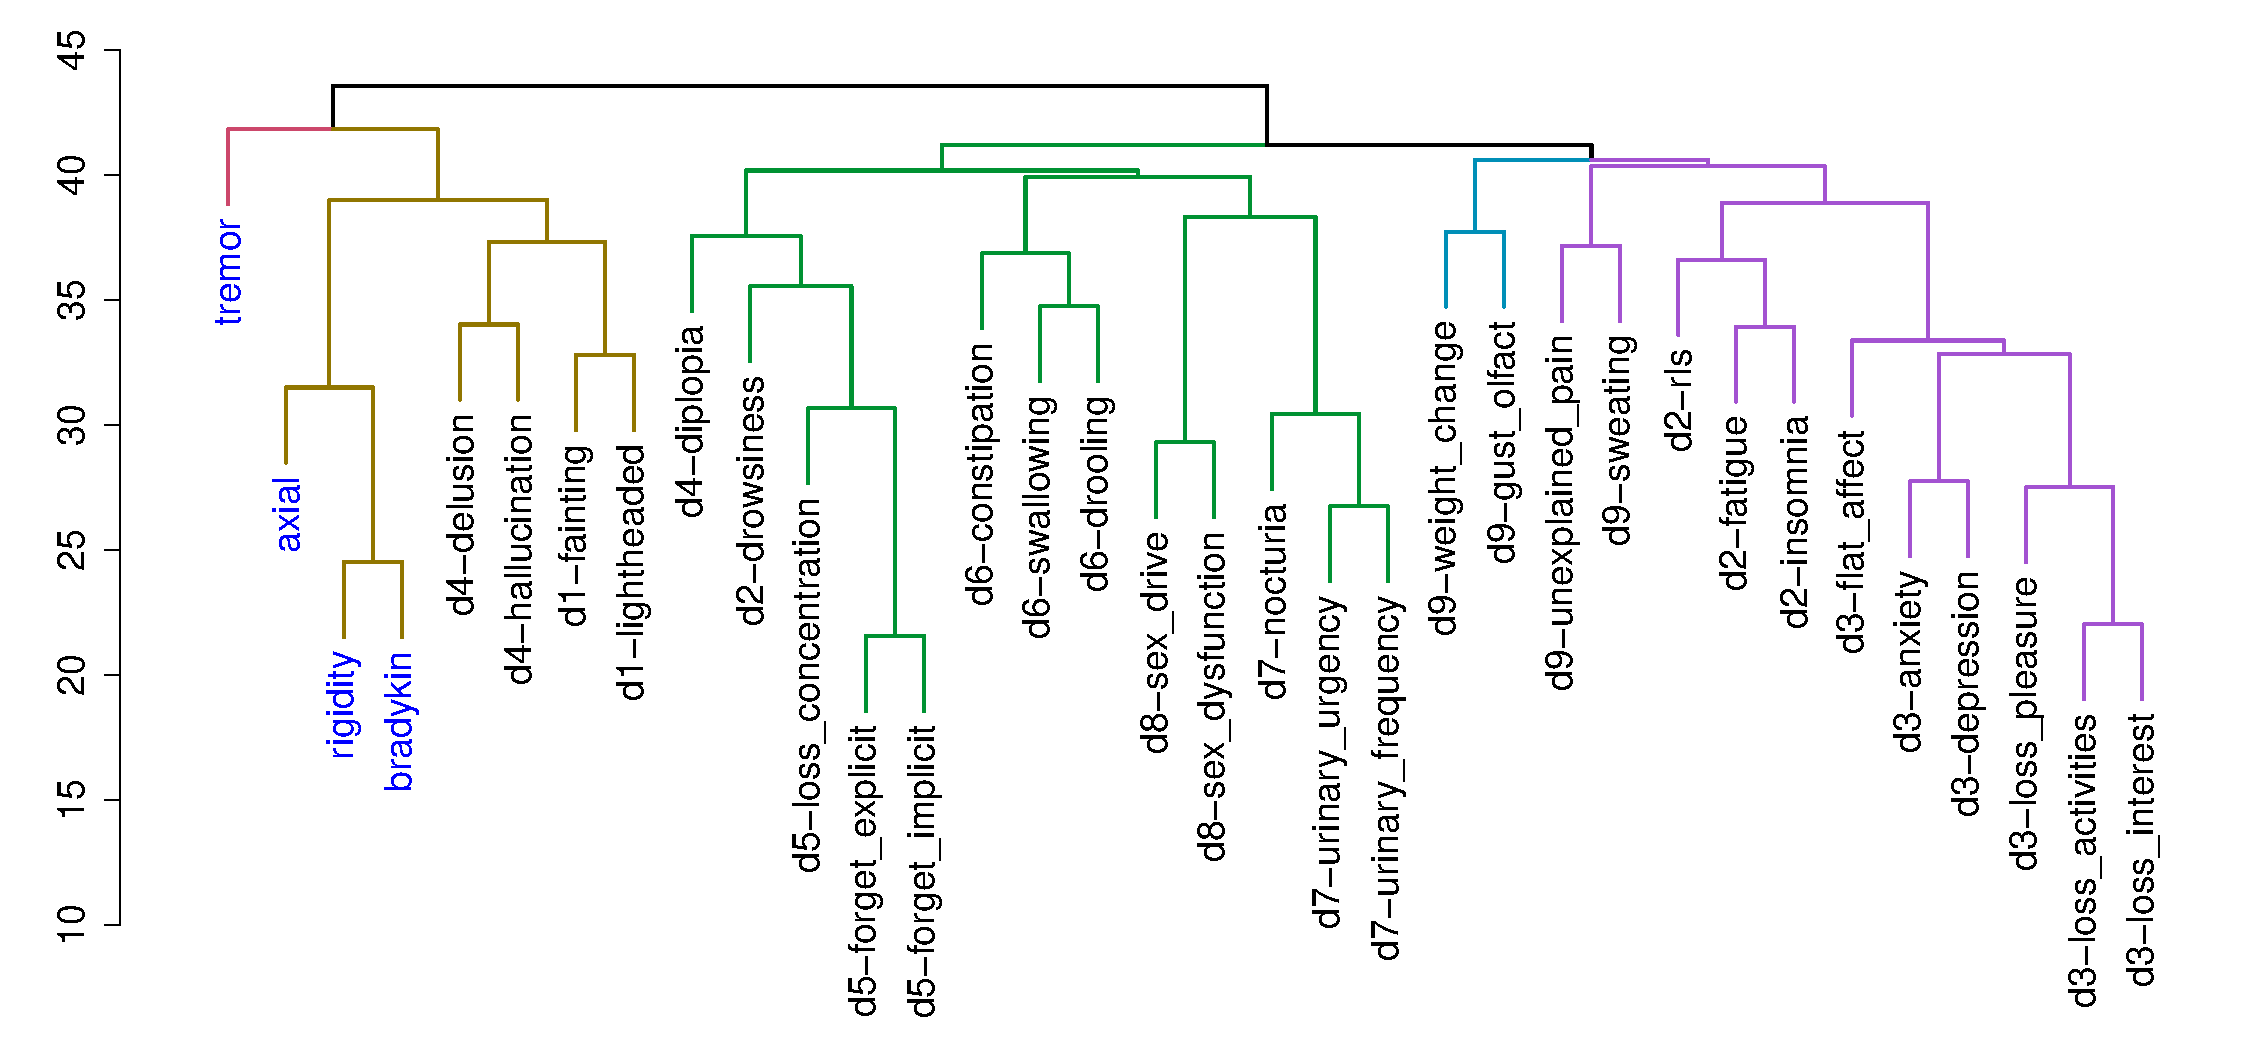
\includegraphics[width=\linewidth]{nms30m-colhc-pub.pdf}
  \caption{Hierarchical clustering of motor (blue) and nonmotor (black) symptoms. Symptoms are
  labeled with their name and corresponding domain number. Dendrogram colored with 4 clusters.}
  \label{fig:hc}
\end{figure*}

\section{Discussion}

$k$-means clustering on this Parkinsons' Disease data set reveals clusters that confirm previous
findings in the field, mainly van Rooden et al.\cite{vanrooden10} and the identification of four
subtypes of Parkinson's disease: mild, nonmotor-predominant, motor-predominant, and severe.  van
Rooden's work was done with a separate dataset using a different modeling method
(expectation-maximization), and this investigation independently confirms these subtype
classifications. Unlike van Rooden, mean disease durations differences do exist between subtypes 1
(mild) and 4 (severe), likely due to further development of the disease, although the differences
between 2 and 3 (nonmotor/motor predominated) subtypes are insignificant
(Table~\ref{tab:tukeyhsd}), suggesting different developmental paths of the disease.

Overall, little information was found in pdonset,
durat\_pd, or current age, according to Tables~\ref{tab:tukeyhsd}
and~\ref{tab:info_gain}.  Mean ages were similar for subgroups 1, 2, and 3 ($p >
0.05$), but different for the severe subtype 4, which makes sense given that
patients in 4 also have longer disease durations. Specifically, clusters 1 and
4 seem to be phenotypically quite similar, except at different stages of
disease progression, given cluster 4's higher age and durat\_pd scores.

However, clusters 2 and 3 clearly show different disease progression, one in
the motor direction, and one in the nonmotor. Both groups have similar age,
pdonset, and durat\_pd scores, but differ wildly in symptomatic expression.
Cluster 2 is dominated by a high prevalence of nonmotor symptoms, such as
nms\_d2, nms\_d3, nms\_d7, and nms\_d9. Cluster 3, however, is dominated by a
high prevalence of motor symptoms, while most motor symptoms are similar to the
mild cluster 1. Of note is that the tremor population mean
is the highest cluster mean, even higher than the severe subtype 4. This
motor-dominant cluster may thus overlap with Ma's tremor dominant/slow
progression cluster\cite{ma15}.

Generally, given stable pdonset scores and predictably increasing durat\_pd
scores for clusters 1 and 4, Ma et al's rapid disease
progression/late onset and tremor dominant/slow progression clusters
\cite{ma15} were mostly not found in this dataset, save for the tremor-dominant
motor cluster.

The most important nonmotor symptoms in determining these clusters were nms\_d2
(sleep) and nms\_d3 (mood/cognition), which echo findings of Fereshtehnejad's
longitudinal study\cite{fereshtehnejad15} and are similar to Sauerbier's
identification of sleep dominant and cognitive dominant clinical NMS subtypes\cite{sauerbier15}.
Compared to Erro et al.\cite{erro13}, nonmotor/motor
dominant subtypes were indeed found, but an additional subgroup with relatively
severe levels of both motor and nonmotor symptoms were found. Erro's benign
subtype groups possibly overlap with the mild cluster 1 found in this
investigation.

\subsection{Nonmotor subtype: clustering and modeling}
Nonmotor symptoms nms\_d2 and nms\_d3 became critical not only in
classification trees distinguishing between the various symptoms but in the
nonmotor-predominant subgroup itself. In $k$-means subdivision of the
nonmotor-dominant subtype where $k = 2$ and $k = 3$, opposite trends were
confirmed with nms\_d2 and nms\_d3 symptoms. Similarly, in the 2 and 4 vs rest
decision tree (Figure~\ref{fig:dtree-2and4va-pruned}), nms\_d2 and nms\_d3 nodes were
used to differentiate various categories of nomotor-dominant patients.
When $k = 3$, the subtype with the highest nms\_d2 scores and lowest
nms\_d3 scores had by far the highest axial scores, nms\_d6 (gastrointestinal)
scores, and nms\_d7 (urinary) scores. Thus subtype 3 of the nonmotor-dominated
group could include patients falling into the cognitive/depression-dominant or
autonomic dominant subtypes.

Despite the variety in symptomatic expression in this nonmotor group, what
seems most consistent is the presence of nms\_d9 (miscellaneous) nonmotor
symptoms, as it is used as the root node of the 2 vs all decision tree
(Figure~\ref{fig:2va}) and the 2 and 4 vs rest decision tree
(Figure~\ref{fig:dtree-2and4va-pruned}).

It remains to be seen whether these classification models, especially the one-vs-all decision
trees, are useful in clinical practice.

\subsection{New conclusions}
\label{ssec:newconc}

First, the longitudinal analysis gives more insight into the clusters found when clustering on
nms\_d\{1-9\}. According to Figure~\ref{fig:longcorr}, most symptoms are highly correlated, with PD
duration, but notably, mood/cognition symptoms (nms9, nms10, nms12) and tremor are not correlated
highly with PD duration. The differences in disease progression can be seen by the corresponding
graphs, Figures~\ref{fig:nms9-multi} and~\ref{fig:nms10-multi}. In both graphs, what is interesting
is that Subtype 2 (Nonmotor-Dominant) starts at higher scores for nms\_9 and nms\_10, thus
indicating that these patients' subtype is can be determined early in PD duration from depressive
symptom score. Similarly, when examining Subtype 3 (Motor-dominant) in
Figure~\ref{fig:tremor-multi}, the mean tremor score is substantially higher from PD onset.
Interestingly, Subtype 4 (Severe) generally starts at lower tremor and motor scores during disease
onset (Figure~\ref{fig:cisitot-multi}), but then rises sharply, exceeding other Subtypes. More evidence
that tremor is a unique motor symptom is located in Figure~\ref{fig:nms30m-colhc}, where it is the most
distant symptom from all other symptoms.

When examining all 30 symptoms, more evidence is given that the previously-discovered Subtype
2 (Nonmotor-Dominant) may be primarily characterized by high depressive symptoms. By graphing the
30 subtypes attached to the original clustering, as in Figure~\ref{fig:d9to30}, the mean scores of
nms8, nms9, and nms10 for Subtype 2 are substantially higher than Subtypes 1 and 3.

Indeed, PCA on the 30 nonmotor symptoms identifies the second-most prominent component as a general
mood/cognition component, and $k$-means clustering on the 30 symptoms only
(Figure~\ref{fig:nms30m-k4-heatmap-improved}) divides the 1000 patients into four slightly
different groups, a mild, average, depression-dominant, and severe group.

The Gaussian mixture model identified in Figure~\ref{fig:nms30m-mclust-heatmap-improved} fragments
the previously-discovered clusters into more groups. Here, a wide variety of specialized subtypes
of PD are displayed, including insomnia, urinary, motor, nonmotor, and depression-dominant groups,
as well as the expected mild, average, and severe subtypes. It is likely that the previous analysis
with only nms\_d\{1-9\} combined most of those specialized groups into the more general
nonmotor-dominant Subtype 2.

It's intuitive that a Depression-Dominant group emerges when clustering on nms\{1-30\}, since
domain 3 consists of 5 separate measures. Thus, any high expression of depressive symptoms is
magnified in clustering, since the symptoms are highly similar (Figure~\ref{fig:nms30m-colhc}) and
treated with equal weight. Once again reinforcing what was discovered previously, depressive
symptoms have been shown to be very important in determining subtypes of PD.

\section{Supplementary Material}
\section{References}

\bibliography{manuscript}

\end{document}
